\section{Experiment P2G: continuing global position reference}
\label{sec:p2g}
\subsection{Purpose and matched comparison}
P2G is a separate extension to the infrastructure-free P2A--P2F sequence. It asks whether a continuing global position observation of one moving node can reduce common drift in the other nodes through their UWB links. Known initial positions alone were already present in P2A. The new information is the reference position \emph{throughout} the run.

The four original paths, 60 s duration, 100 Hz IMU, reference sensor amplitudes, frozen process covariance, clean ranges, initialization errors, and 20 matched seeds remain unchanged. Node 1 becomes the position reference but keeps its IMU and estimated velocity and yaw. Only its position is observed; true velocity, true yaw, and the other nodes' true positions are never supplied to the estimator after initialization. The same six links and cyclic timing are used at budgets \(0,180,360,720,3600\).

Every headline fleet, worst-node, centroid, relative-shape, and yaw metric is evaluated on \textbf{the same three non-reference nodes, 2--4}, including the unanchored control. This prevents a zero-error reference from mechanically lowering reported fleet error. Centroid and shape are recomputed for these three nodes, with no global alignment. Their numerical values therefore differ from the four-node P2F metrics; only matched P2G conditions are directly compared.

\subsection{Reference cases, estimator, and cost}
\begin{table}[htbp]
\centering\small
\begin{tabular}{lrrl}
\toprule
Reference case & Rate (Hz) & Updates & Position observation\\
\midrule
Unanchored & 0 & 0 & None after initialization\\
Exact & 100 & 6000 & True node-1 position\\
Noisy & 1 & 60 & Gaussian, 0.10 m per axis\\
Noisy with outage & 1 & 50 & Same reports, absent in $[20,30)$ s\\
\bottomrule
\end{tabular}
\caption{P2G reference service over 60 s. Counts exclude known initial poses. Noisy reports occur at integer seconds and resume at 30 s after the outage. UWB and IMU remain available throughout.}
\label{tab:p2g_cases}
\end{table}

The noisy report is \(\bm z_k=\bm p_1(k)+\bm\nu_k\), with independent \(\bm\nu_k\sim\mathcal N(0,0.01I_2)\) in square metres. Its RNG stream is separate from initialization, IMU, and UWB; the uninterrupted and outage cases reuse the same available reports. The ideal case represents position information available at every integration step, rather than a realistic external device. Comparing it with noisy 1 Hz reports changes both accuracy and update rate, so their difference cannot isolate either effect.

At an available report, the full joint state and covariance are conditioned on node 1's two position coordinates. With the selection matrix \(H_p\),
\begin{align}
K_p &= P^-H_p^\top(H_pP^-H_p^\top+R_p)^{-1},\\
\hat{\bm x}^+ &= \hat{\bm x}^-+K_p(\bm z-H_p\hat{\bm x}^-),\\
P^+ &= (I-K_pH_p)P^-(I-K_pH_p)^\top+K_pR_pK_p^\top.
\end{align}
For exact position, \(R_p=0\); node 1's position is enforced exactly and corresponding covariance rows and columns become zero. Velocity and yaw remain estimates and receive only covariance-mediated corrections. Each step applies IMU prediction, then available position conditioning, then UWB. Cross-node covariance and range observations transfer global information to the other nodes. Without UWB, those nodes remain disconnected from the reference information.

Cost is reported as \emph{two separate counts}: attempted undirected UWB exchanges and reference updates. At every fixed UWB budget, all reference cases have identical UWB timing and measurements. All attempts are received and accepted; there is no gate or range corruption. The reference source and delivery network are not modeled, so equal UWB count is not equal total communication or energy. The ideal case is an ideal information benchmark, not a proved estimator-error lower bound.

\subsection{Verification and statistical treatment}
The campaign contains 400 simulations: four cases, five budgets, and 20 seeds. All 100 unanchored four-node endpoints reproduce the inherited P2E reference results at \(10^{-10}\) tolerance. Every reference constraint and transaction count is checked, as is the squared-error decomposition into centroid and relative-shape contributions for three nodes. At zero UWB, non-reference state histories are byte-identical in every reference condition to the unanchored control. Unit checks verify noisy and exact linear-Gaussian conditioning, transfer through cross covariance, positive-semidefinite covariance, and outage masks; existing Phase-2 checks pass after the estimator extension.

Whole-run RMSE uses all 6001 time indices. Means and sample standard deviations are calculated over seeds, empirical p95 uses linear interpolation of the 20 seed-level trajectory RMSE values, and paired intervals use 30000 bootstrap resamples. Intervals remain descriptive and unadjusted for multiple comparisons. The \textbf{0.10 m target now concerns absolute three-node fleet RMSE}, distinct from P2F's relative-shape target. Smallest budgets denote tested crossings only, with no inference within the large 720--3600 gap.

\subsection{Absolute accuracy changes substantially; shape changes little}
\begin{table}[htbp]
\centering\small
\begin{tabular}{lrrrr}
\toprule
At 360 UWB attempts & Fleet mean $\pm$ SD & Centroid & Shape & Worst\\
 & \multicolumn{4}{c}{Three-node position RMSE (m)}\\
\midrule
Unanchored & $1.0613\pm0.4488$ & 1.0576 & 0.0766 & 1.0803\\
Exact reference & $0.1183\pm0.0243$ & 0.0893 & 0.0763 & 0.1391\\
Noisy 1 Hz & $0.1313\pm0.0261$ & 0.1041 & 0.0779 & 0.1519\\
Noisy with outage & $0.1319\pm0.0259$ & 0.1047 & 0.0779 & 0.1517\\
\bottomrule
\end{tabular}
\caption{P2G matched 360-attempt comparison; centroid, shape, and worst columns are means over seeds. Reference updates are respectively 0, 6000, 60, and 50.}
\label{tab:p2g_360}
\end{table}

At 360 attempts, exact position reduces mean absolute fleet RMSE by 0.9430 m, about 88.9\%, with improvement in all 20 seeds. The paired exact-minus-unanchored 95\% interval is \([-1.1409,-0.7614]\) m. Noisy 1 Hz reports also improve every seed, with paired mean \(-0.9300\) m and interval \([-1.1289,-0.7477]\) m. Every reference condition improves every seed at every positive tested UWB budget. At zero UWB all conditions retain the identical non-reference fleet RMSE, \(2.3198\pm0.6425\) m: an observed reference must be linked to the other nodes to benefit them.

\begin{figure}[htbp]
\centering
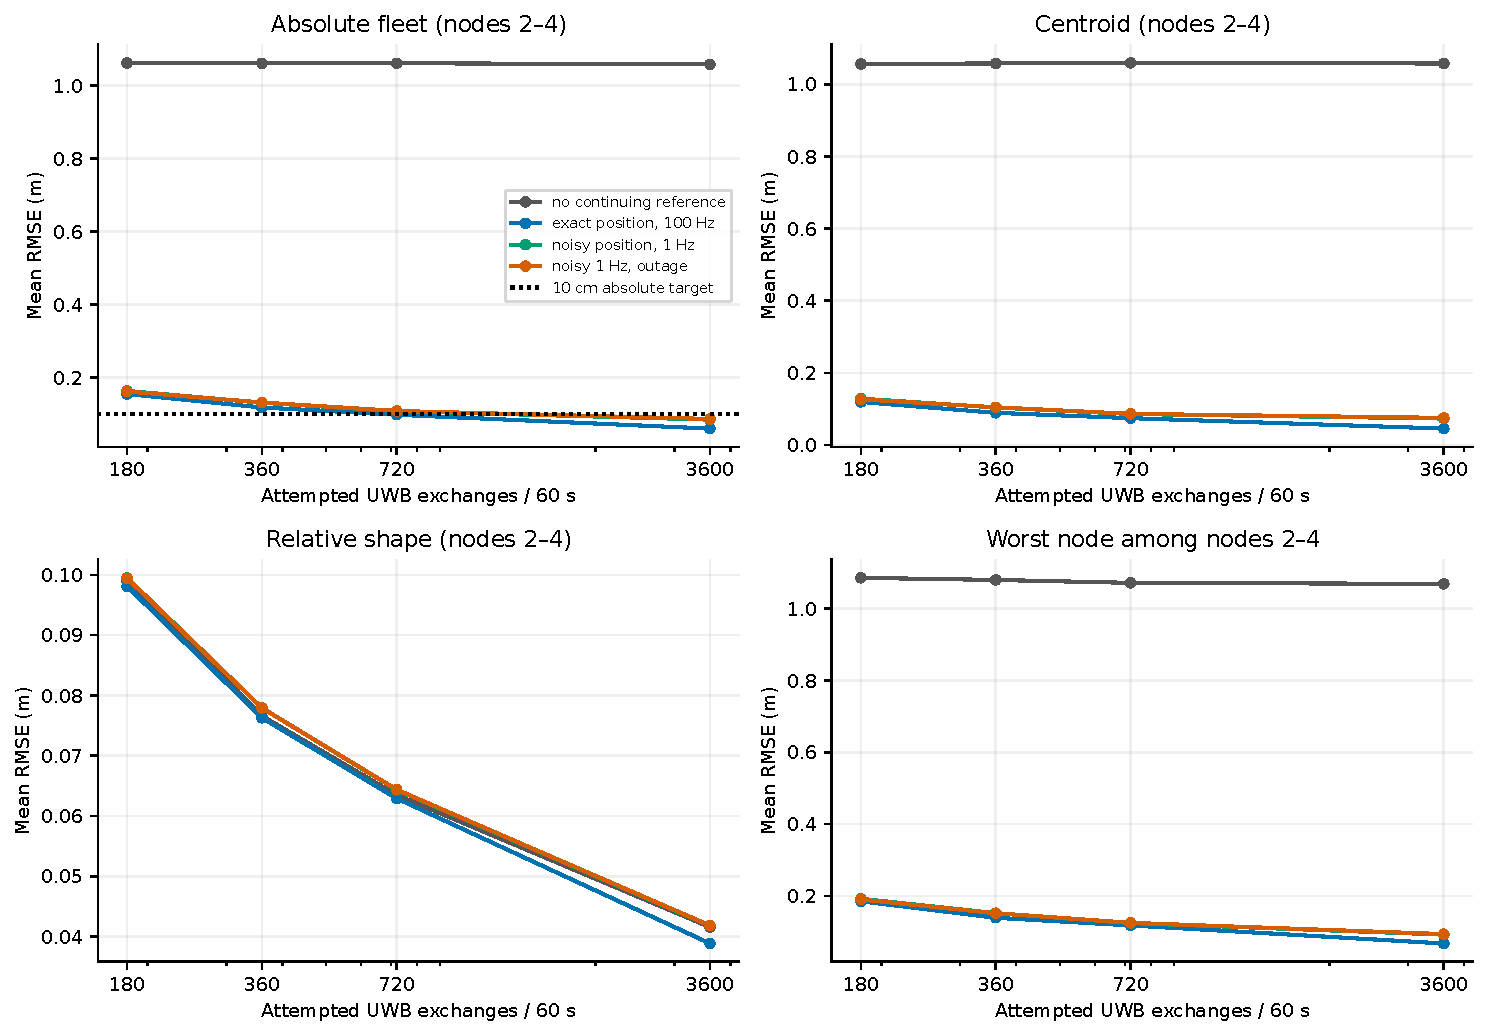
\includegraphics[width=0.98\textwidth]{figures/phase2/p2g_budget_curves.pdf}
\caption{P2G conditional mean accuracy versus attempted UWB budget, scoring nodes 2--4 throughout. Reference-update cost differs between curves (Table~\ref{tab:p2g_cases}). Zero-UWB is retained numerically and omitted from the logarithmic axis. Connecting lines do not imply tested intermediate budgets.}
\label{fig:p2g_budget}
\end{figure}

The large absolute improvement is primarily a centroid effect, not a new relative-shape gain. At 360 attempts, exact reference changes mean shape by only \(-0.00031\) m, with paired interval \([-0.00273,0.00195]\) m and improvement in 9/20 seeds. Noisy reports change it by \(+0.00133\) m, interval \([-0.00112,0.00369]\) m. Thus the geometry was already comparatively accurate; continuing global information constrains drift that pairwise distances alone cannot observe directly. At full communication exact reference does improve shape by 2.72 mm, interval \([-4.25,-1.21]\) mm, but this remains small relative to its absolute-position benefit.

\begin{figure}[htbp]
\centering
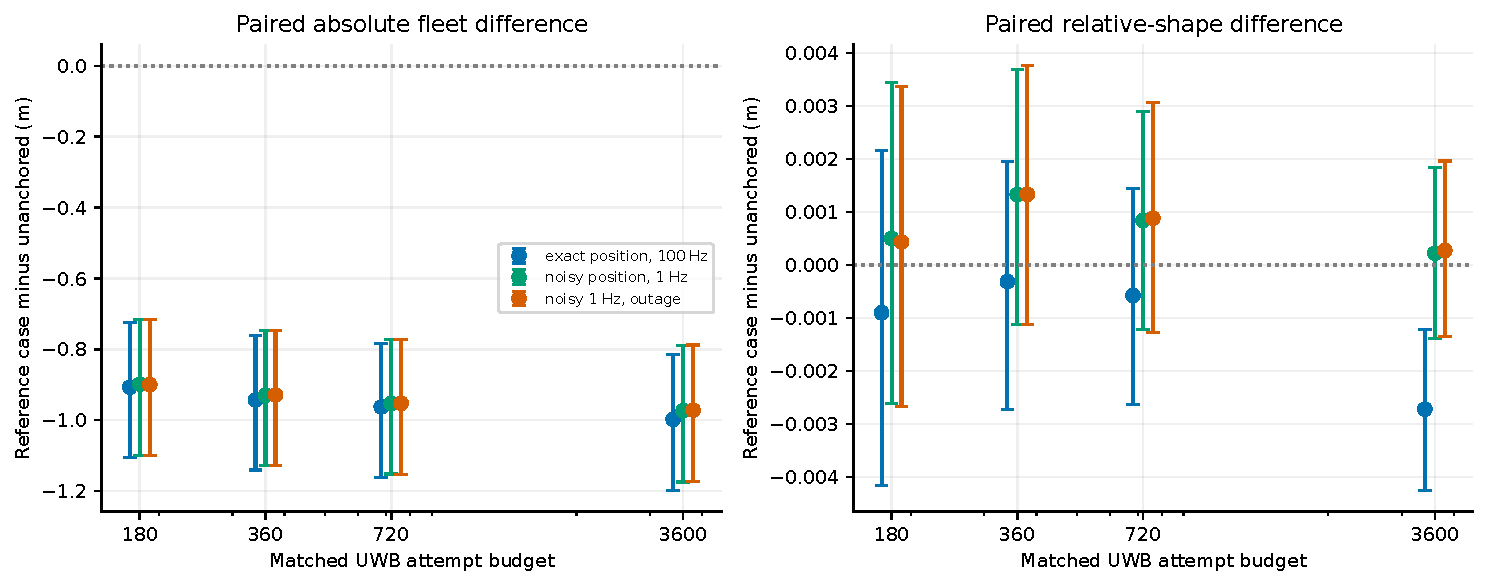
\includegraphics[width=\textwidth]{figures/phase2/p2g_paired_differences.pdf}
\caption{Paired case-minus-unanchored differences over the same seeds and UWB schedules. Negative means favor the reference case. Bars are descriptive, unadjusted bootstrap 95\% intervals. Horizontal offsets distinguish cases at the same attempted budget. Absolute benefits are large; shape differences are small.}
\label{fig:p2g_pairs}
\end{figure}

\subsection{Absolute target and imperfect reference availability}
\begin{table}[htbp]
\centering\small
\begin{tabular}{lrrrr}
\toprule
Reference case & Mean target & p95 target & Passing seeds$^*$ & Full p95 (m)\\
\midrule
Unanchored & --- & --- & --- & 1.6405\\
Exact & 720 & 3600 & 10/20 & 0.0713\\
Noisy 1 Hz & 3600 & --- & 17/20 & 0.1048\\
Noisy with outage & 3600 & --- & 16/20 & 0.1096\\
\bottomrule
\end{tabular}
\caption{Smallest tested UWB budget meeting the 0.10 m absolute fleet target on nodes 2--4. $^*$Passing seeds at the mean-target budget. A dash indicates no crossing at a tested budget. Reference costs remain separate.}
\label{tab:p2g_target}
\end{table}

Exact reference reaches mean absolute RMSE 0.0984 m at 720 attempts, but only 10/20 seeds pass and p95 remains 0.1269 m. At 3600 its mean is 0.0604 m, all seeds pass, and p95 is 0.0713 m. Noisy reports reach mean 0.0851 m at 3600, but their p95 0.1048 m narrowly misses the criterion. Therefore a mean target crossing does not establish consistent 10 cm absolute accuracy, even with continuing external position information. Initial velocity transients and remaining geometry/yaw uncertainty still contribute.

\begin{figure}[htbp]
\centering
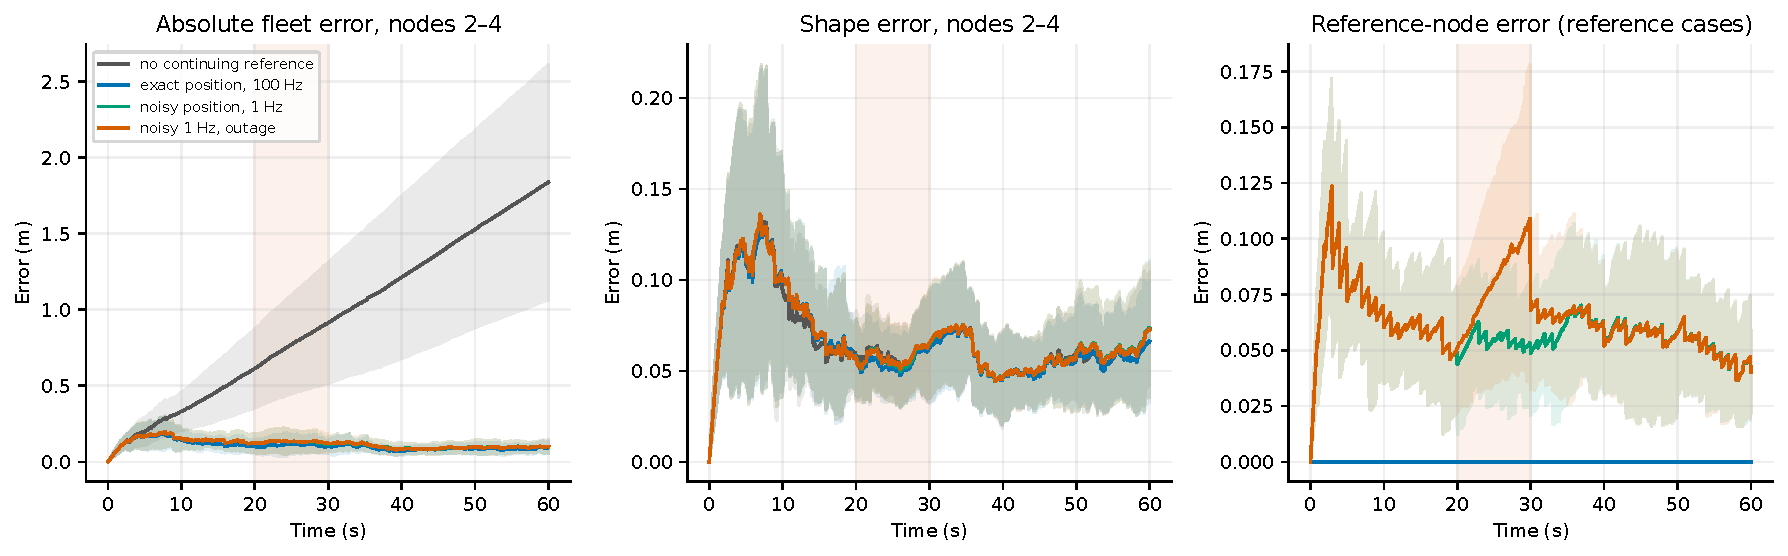
\includegraphics[width=\textwidth]{figures/phase2/p2g_time_profiles.pdf}
\caption{P2G at 360 UWB attempts: mean instantaneous errors with one sample standard-deviation envelope over seeds, sampled at 10 Hz. Lower bands are clipped at zero. The shaded 20--30 s interval applies only to the noisy-outage condition. The right panel shows reference cases only. Reference-node error is a diagnostic and is excluded from headline fleet and shape errors.}
\label{fig:p2g_time}
\end{figure}

The specified 10 s reference outage has little effect on whole-run error: the outage increases noisy fleet RMSE by \(+0.00059\) m at 360 attempts, paired interval \([-0.00130,0.00257]\) m, and \(+0.00169\) m at 3600, interval \([-0.00049,0.00392]\) m. The outage is visible locally: over the sampled \([20,30)\) s window at 360, average instantaneous reference error rises from 0.0539 to 0.0797 m, whereas three-node fleet error changes from 0.1306 to 0.1319 m. These window averages use 10 Hz instantaneous profiles and are not trajectory RMSE. Reports resume at 30 s and reference accuracy recovers. This evidence does not establish robustness to longer, repeated, or differently placed outages.

\subsection{Interpretation and next decision}
P2G supports the proposed global-reference extension: one continuously localized moving node can substantially improve the absolute positions of other nodes through their existing UWB links. The effect is distinct from P2C's small clean pair-selection gains. It changes the application assumptions and introduces a reference service whose uncertainty, availability, and cost must be stated explicitly. One position reference does not provide every orientation constraint or prove general observability; the results remain specific to these paths, initial conditions, and estimator.

P2A--P2G are now complete. The next scientific decision is the intended operating mode: infrastructure-free relative geometry or globally referenced absolute localization. A deployment-focused continuation should choose a reference source, realistic noise/report availability, an accuracy criterion, and a total cost model. Reliability-aware scheduling or bias-state estimation should remain distinct experiments, rather than being mixed into the current comparison.

Use \texttt{configs/phase2g.yaml} and run the following Python scripts from the repository root:
\begin{quote}\footnotesize
\url{experiments/run_phase2g.py}\\
\url{experiments/generate_phase2g_figures.py}
\end{quote}
The seed metrics, paired differences, time profiles, representative trajectories, endpoint audit, and complete statistical summary are stored under \texttt{results/phase2/p2g/}. Atomic per-seed checkpoints support resumption, with a configuration and implementation fingerprint to reject stale results.
